\section{Method}

\begin{figure}
    \centering
    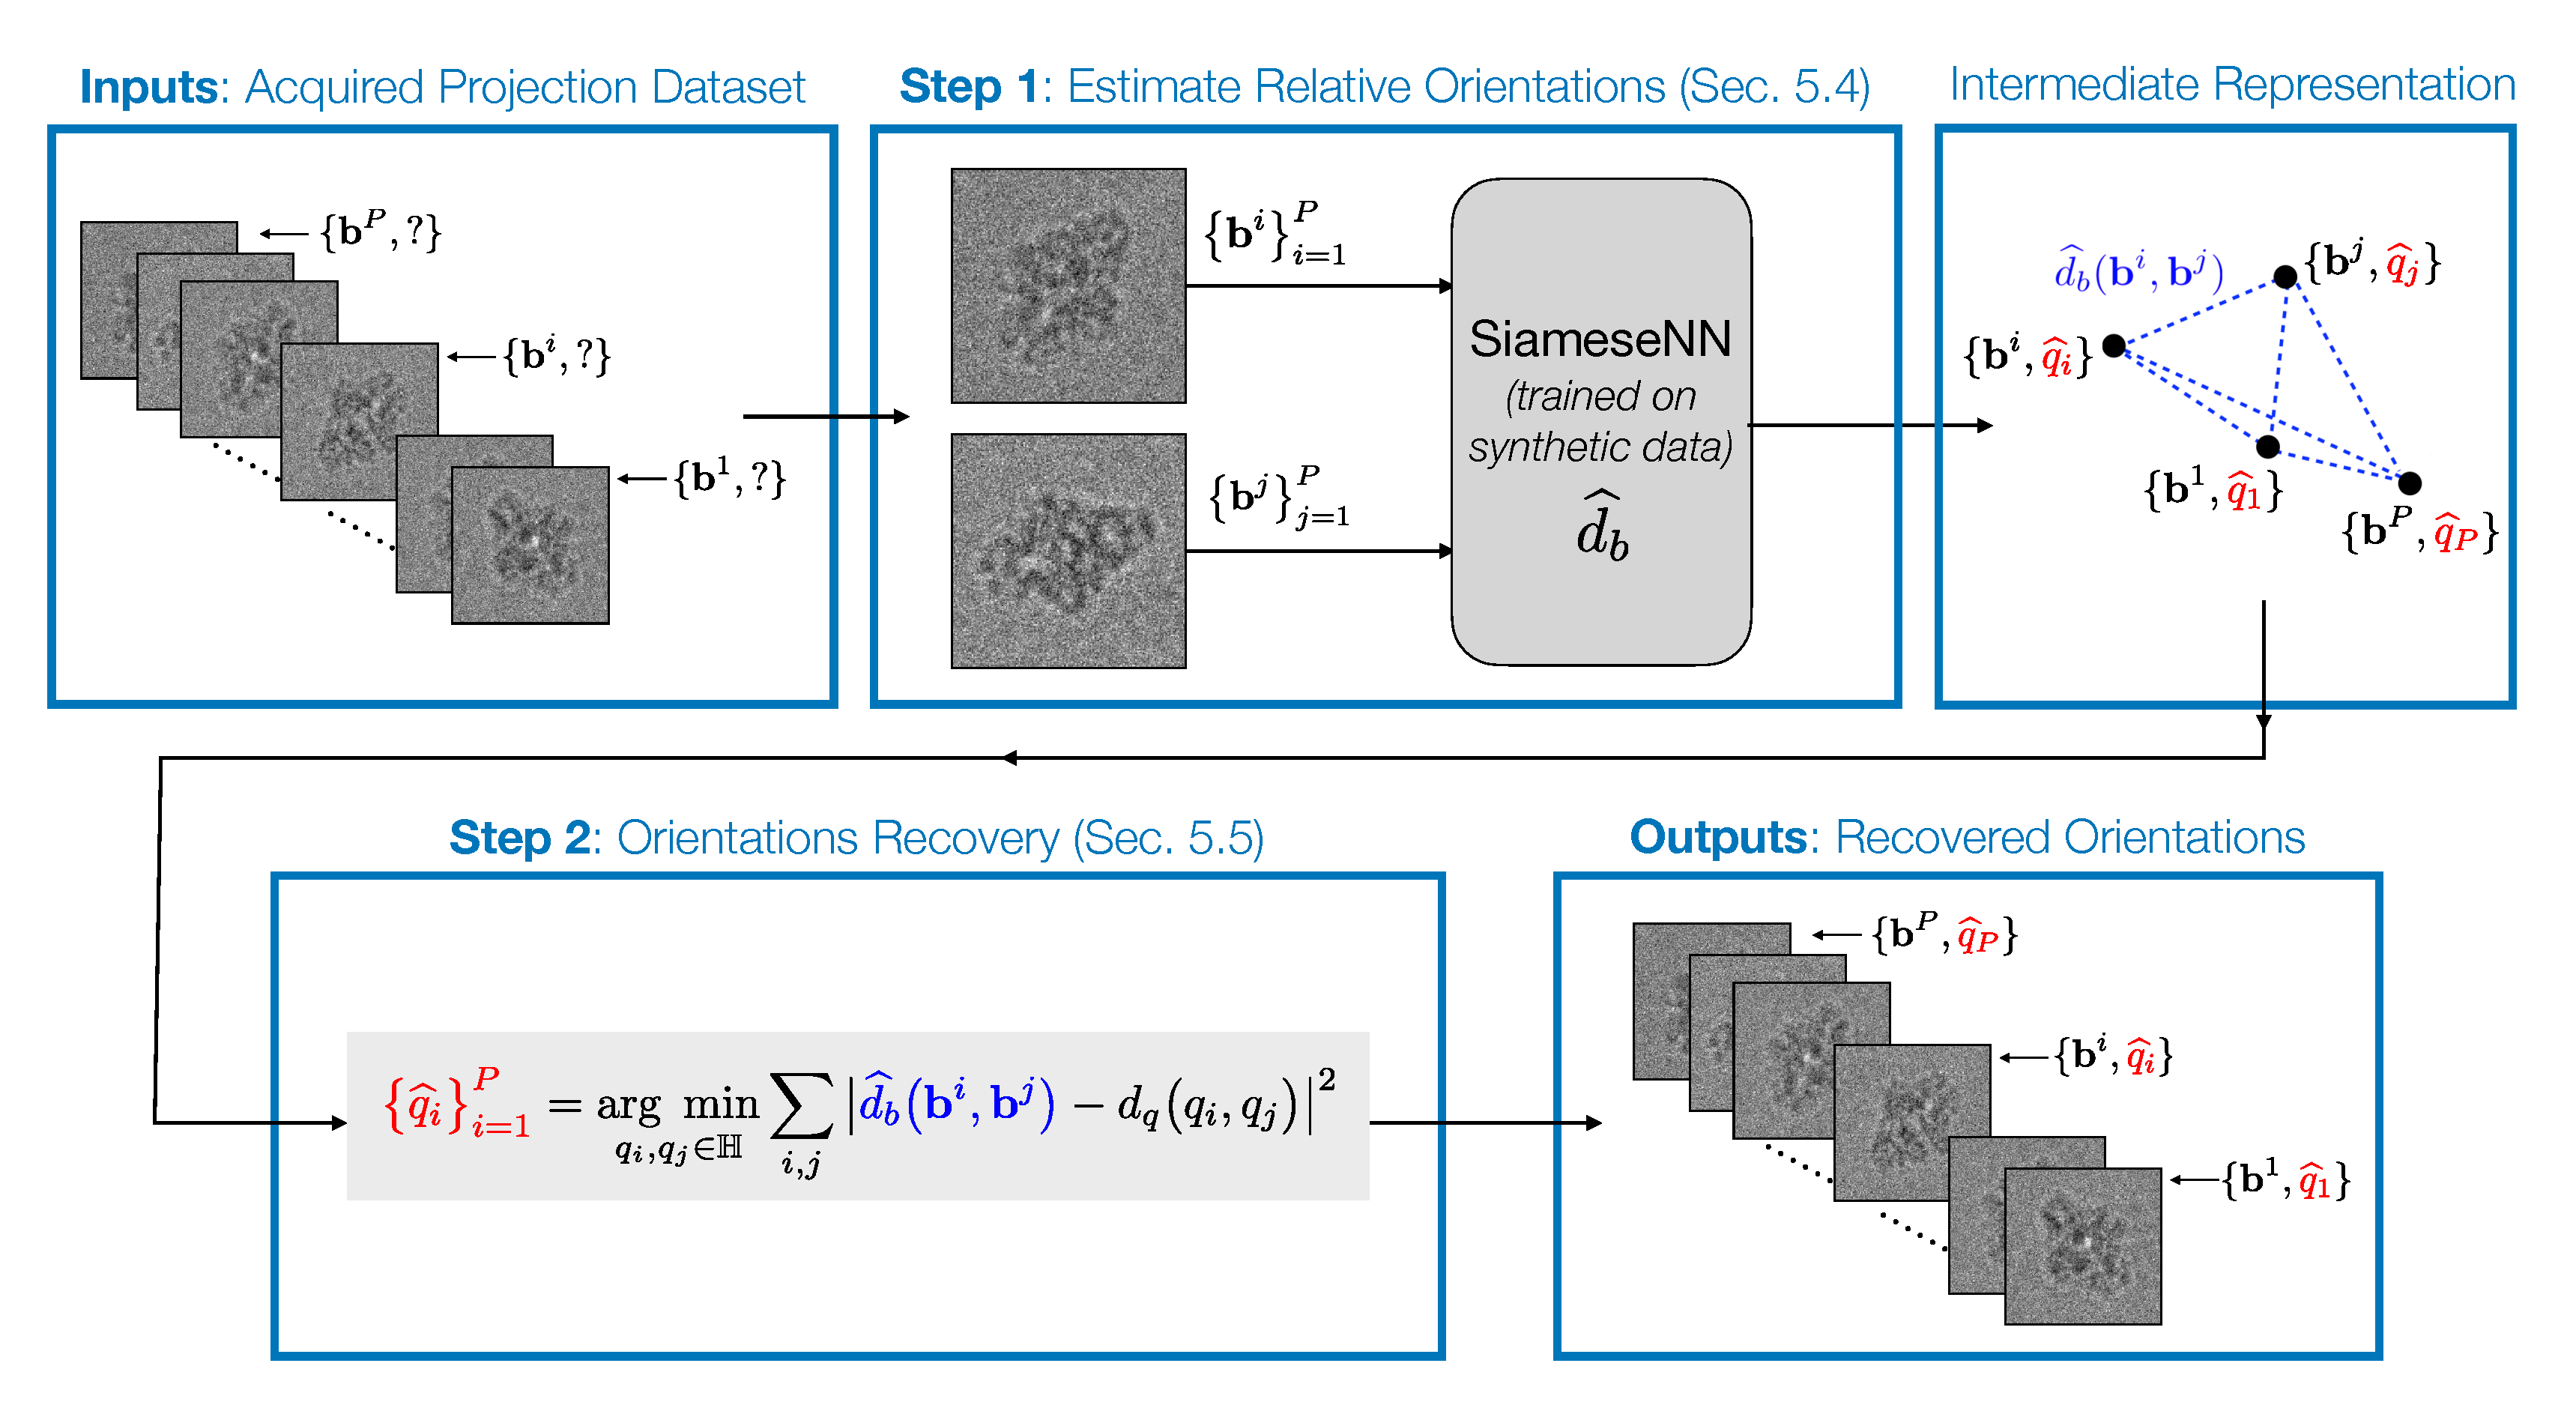
\includegraphics[width=\textwidth]{schematic_overview}
    \caption{
        Method overview.
        We denote the $p$th projection by $\mathbf{b}^p$ and its orientation by $q_p$.
        $d_q$ denotes the distance between two orientations and $\widehat{d}_b$ the estimated distance between two projections, implemented as a SiameseNN.
        Our method is made of two steps: (i) estimate distances between pairs of projections, and (ii) recover orientations from the estimated distances.
        % Our method effectively (i) estimates a metric space, then (ii) embed it in the space of 3D orientations, $\SO(3)$.
        \todo{Update sections in figure.}
        \todo{Update titles: Step 1: estimate distances. Step 2: recover orientations.}
        \mdeff{It would be amazing to have a visual of the embedding made in step 2: finding points in SO(3) such that the geodesic distances between them are the estimated distances. As we can't see SO(3) / $S^3$, we could try with $S^2$, which is a subset/projection.}
    }
    \label{fig:schematic:overview}
\end{figure}

The more similar two projections are, the more likely they originate from two 3D particles that adopted close orientations.\footnote{Up to protein symmetries, which we discuss later.}
From this observation, which guides a number of applications in SPA like~\cite{penczek1994ribosome} \mdeff{(would be better to have a review ref with multiple applications)}, we propose to (i) estimate a metric space from projections, then (ii) realize it in the space of 3D orientations.
%to embed it on the space of 3D orientations, $\SO(3)$.
% In practice, our method consists of: (i) estimate the distance between pairs of projections, and (ii) recover
% \mdeff{maybe too repetitive with figure caption}
Our method is illustrated in \figref{schematic:overview}.

\todo{Zoom on orientation recovery. Merge and shorten.}
\mdeff{Story: recovery is the minimization of an objective function. Convex in the Euclidean case, unknown for $\SO(3)$ but hopeful because locally Euclidean and empirically works with SGD.}
Methods are standard for dimensionality reduction and data visualization, whose goal is to transform high-dimensional data to a low-dimensional space while preserving distances / metric / structure.
(i) build graph, (ii) realize / embed it in some ambient space
Laplacian eigenmaps, multi-dimensional scaling (MDS), Isomap, LLE, t-SNE, UMAP are well-known examples.
The embedding of distance matrices is well-studied for Euclidean embedding spaces, where the embedding is given by the eigenvectors of the distance matrix.
The task of recovering points based on their relative distances has been extensively studied in the literature, mostly within the framework of dimensionality reduction and primarily for the case of \textit{Euclidean} embedding spaces\footnote{An ``embedding space'' corresponds to the (often lower-dimensional) space in which data is embedded, \textit{i.e.}, mapped to in such a way that the relative distances between its points are preserved as much as possible.}~\cite{belkin2003laplacian,kruskal1978multidimensional, maaten2008visualizing, mcinnes2018umap,dokmanic2015euclidean}.
In~\cite{dokmanic2015euclidean}, the embedding space being Euclidean, the theoretical framework of the Euclidean distance matrices (EDMs) guarantees that one can retrieve the desired points from the collected distances.
In our case, as we shall shortly explain, we aim to embed the estimated relative orientations on $\SO(3)$, the space of 3D rotations.
the space of 3D orientations.
Despite this lack of theoretical guarantees, we are able to appropriately minimize our objective function using a gradient-based algorithm, as we experimentally demonstrate in \secref{results:orientation-recovery:exact}.
Similarly, we do not know of any theoretical characterization of the behaviour of~\eqnref{orientation-recovery} in ill-posed conditions, such as when pairwise distances are misestimated, for instance.
\todo{hopeful because $\SO(3)$ is locally similar to 3D Euclidean space. Empirically good, see xx}

\todo{Zoom on distance estimation. Merge and shorten.}
In our case, we don't have access to the distances, and must estimate them.
distances that may not be directly measurable:
the similarity between two projections to be a good proxy for their relative orientation, for some meaning of similarity.
Hand-crafted impossible but learn easy.
If the distances are exact geodesic distances between orientations, then orientation recovery will find a perfect realization of the metric space, with zero error.
In practice, distances estimated from projections will only be a proxy of true distances.
Experiment \secref{results:orientation-recovery:sensitivity} shows that a lower distance estimation error translates to a lower orientation recovery error.
Hard to design a distance because the invariants are difficult to specify. Learning is easier because we have data.
Metric learning.
There is no simple way to ``handcraft'' a proxy distance that would robustly predict the similarity between two projections.
Hence, we resort to \textit{learning} this distance function by parametrizing it as a neural network and capitalizing on 1) the public availability of large datasets of 3D atomic models\footnote{\texttt{https://www.ebi.ac.uk/pdbe/emdb}}, and 2) our ability to model the cryo-EM imaging process.
we train a function---parametrized as a neural network---to predict the relative orientation between two projections based on their similarity.
To make such training possible, we capitalize on our ability to model the cryo-EM imaging procedure to generate a large, representative synthetic dataset using publicly available 3D atomic models.
We capitalize on the powerful function approximation capabilities of neural networks and on our ability to faithfully model the cryo-EM imaging process for the generation of training data.
Once the distance learned, it can be used in the aforementioned two-steps method (see \figref{schematic:overview}) for any projection dataset.
SiameseNNs, also termed ``twin networks'', are commonly used in the field of deep metric learning to learn similarity functions~\cite{yi2014deep}.

%\subsection{Unit Quaternions and the Geodesic Distance}
%\subsection{Representation of orientations}
\subsection{Orientation representation}\label{sec:method:orientation-representation}

\todo{Rephrase and shorten.}
\mdeff{The important equations are \eqnref{distance-learning} and \eqnref{orientation-recovery}, then \eqnref{orientation-recovery-error}, \eqnref{distance:orientations}, and \eqnref{distance:projections}. The others must be less prominent for them to shine. Equations are like text: the less the better.}

Orientations $q_p \in \SO(3)$.
\todo{possibilities: 3D rotation matrices, Euler angles, angle-axis, unit quaternions.} \mdeff{@Laurène: could you take a short discussion from your thesis?}

Our method requires the computation of the geodesic distance between two orientations $\mathbf{R}_1, \mathbf{R}_2 \in \SO(3)$, which corresponds to the rotation $\mathbf{R}_* \in \SO(3)$ such that $\mathbf{R}_1 = \mathbf{R}_* \mathbf{R}_2$.

It is standard in SPA to work with Euler angles to describe the orientation of a 3D object in the electron microscope.
More precisely, one relies on the parametrization $\bth=(\theta_1,\theta_2,\theta_3)\in\Omega_\bth$, with $\Omega_\bth=[0;2\pi)\times [0;\pi] \times [0;2\pi)$, to encode the 3D rotation that relates the object coordinate system to the projection coordinate system.

Unfortunately, the relative distance between two rotations $\mathbf{R}(\bth_1)$, $\mathbf{R}(\bth_2)$, parametrized by Euler angles cannot be directly computed from $\bth_1$, $\bth_2$.
It requires the computation of the rotation matrices, which is computationally inefficient\footnote{Another technical challenge with Euler angles is that they suffer from the so-called gimbal lock problem, which arises when $\theta_2=0$ and restricts the number of rotational degrees of freedom to one even though $\theta_1$ and $\theta_3$ have not yet been fixed~\cite{koks2006explorations}.}.
Hence, we resort to a more convenient representation of 3D rotations that relies on unit quaternions.

A quaternion $q\in\mathbb{H}$ takes the form
$q =  a\boldsymbol{1} + b\boldsymbol{i} + c\boldsymbol{j} + d\boldsymbol{k}$,
where $(a,b,c,d) \in \R^4$, and $\boldsymbol{1}$, $\boldsymbol{i}$, $\boldsymbol{j}$, and $\boldsymbol{k}$ are the fundamental quaternion units
\begin{equation*}
    \boldsymbol{1} = \begin{pmatrix} 1 & 0 \\ 0 & 1 \end{pmatrix}, \quad
    \boldsymbol{i} = \begin{pmatrix} i & 0 \\ 0 & -i \end{pmatrix}, \quad
    \boldsymbol{j} = \begin{pmatrix} 0 & 1 \\ -1 & 0 \end{pmatrix}, \quad
    \boldsymbol{k} = \begin{pmatrix} 0 & i \\ i & 0 \end{pmatrix},
\end{equation*}
with $i$ the imaginary unit.
Any quaternion $q$ can thus be represented by its set of coefficients $(a,b,c,d)\in\mathbb{R}^4$.
The algebra $\mathbb{H}$ is similar to the algebra of complex numbers $\mathbb{C}$, with the exception of the multiplication operation being non-commutative.

In this work, we restrict our interest to unit quaternions $q\in\mathbb{U}$, with  $\mathbb{U}=\big\{q\in\mathbb{H} \; \, | \; \,\lvert q \rvert =1\big\}$, which identify the $\mathbb{S}^3$ hypersphere in  $\mathbb{R}^4$.
Unit quaternions concisely and elegantly represent the elements of the $\SO(3)$ group.
More precisely, a unit quaternion $q\in\mathbb{U}$ parametrizes a rotation $\mathbf{R}\in\SO(3)$ through
\begin{equation*}
    \mathbf{R}(q) =\begin{pmatrix}
    a^2+b^2-c^2-d^2 & 2bc-ad & 2bd+2ac  \\
    2bc+2ad & a^2-b^2+c^2d^2 & 2cd-2ab \\
    2bd-2ac & 2cd+2ab & a^2-b^2-c^2+d^2
    \end{pmatrix}.
\end{equation*}

The geodesic distance $d_q:\mathbb{U}\times\mathbb{U}\rightarrow [0,\pi]$ between two unit quaternions $q_i, q_j\in\mathbb{H}$ is then defined as
\begin{equation}
    d_q(q_i, q_j) = 2 \arccos \big(| \langle q_i, q_j \rangle| \big),
    \label{eqn:distance:orientations}
\end{equation}
with the inner product between quaternions given by $\langle q_i, q_j \rangle = a_ia_j+b_ib_j+c_ic_j+d_id_j$.
The distance~\eqnref{distance:orientations} is the shortest distance between $q_i$ and $q_j$ on the surface of $\mathbb{S}^3$.

As $\mathbb{S}^3$ is isomorphic to the universal cover of $\SO(3)$, the geodesic distance corresponds to the magnitude of the relative orientation $\mathbf{R}_*$ between $\mathbf{R}(q_i)$ and $\mathbf{R}(q_j)$ in $\SO(3)$~\cite{huynh2009metrics}.
In other words, the relative distance between two rotations encoded by unit quaternions can be efficiently computed from the unit quaternions themselves through~\eqnref{distance:orientations}, which is of key practical importance for this work.

For the sake of conciseness, we shall use the term ``with orientation~$q$'' to refer to 2D/3D objects considered in an imaging geometry parametrized by $q$.

\subsection{Distance learning}%\label{sec:method:distance-learning}
%\subsection{Metric learning}%\label{sec:method:distance-learning}
%\subsection{Estimating Relative Orientations from Projections}
%\subsection{Relative orientation estimation}
%\subsection{Relative orientation estimation from projections}

\begin{figure}
    \centering
    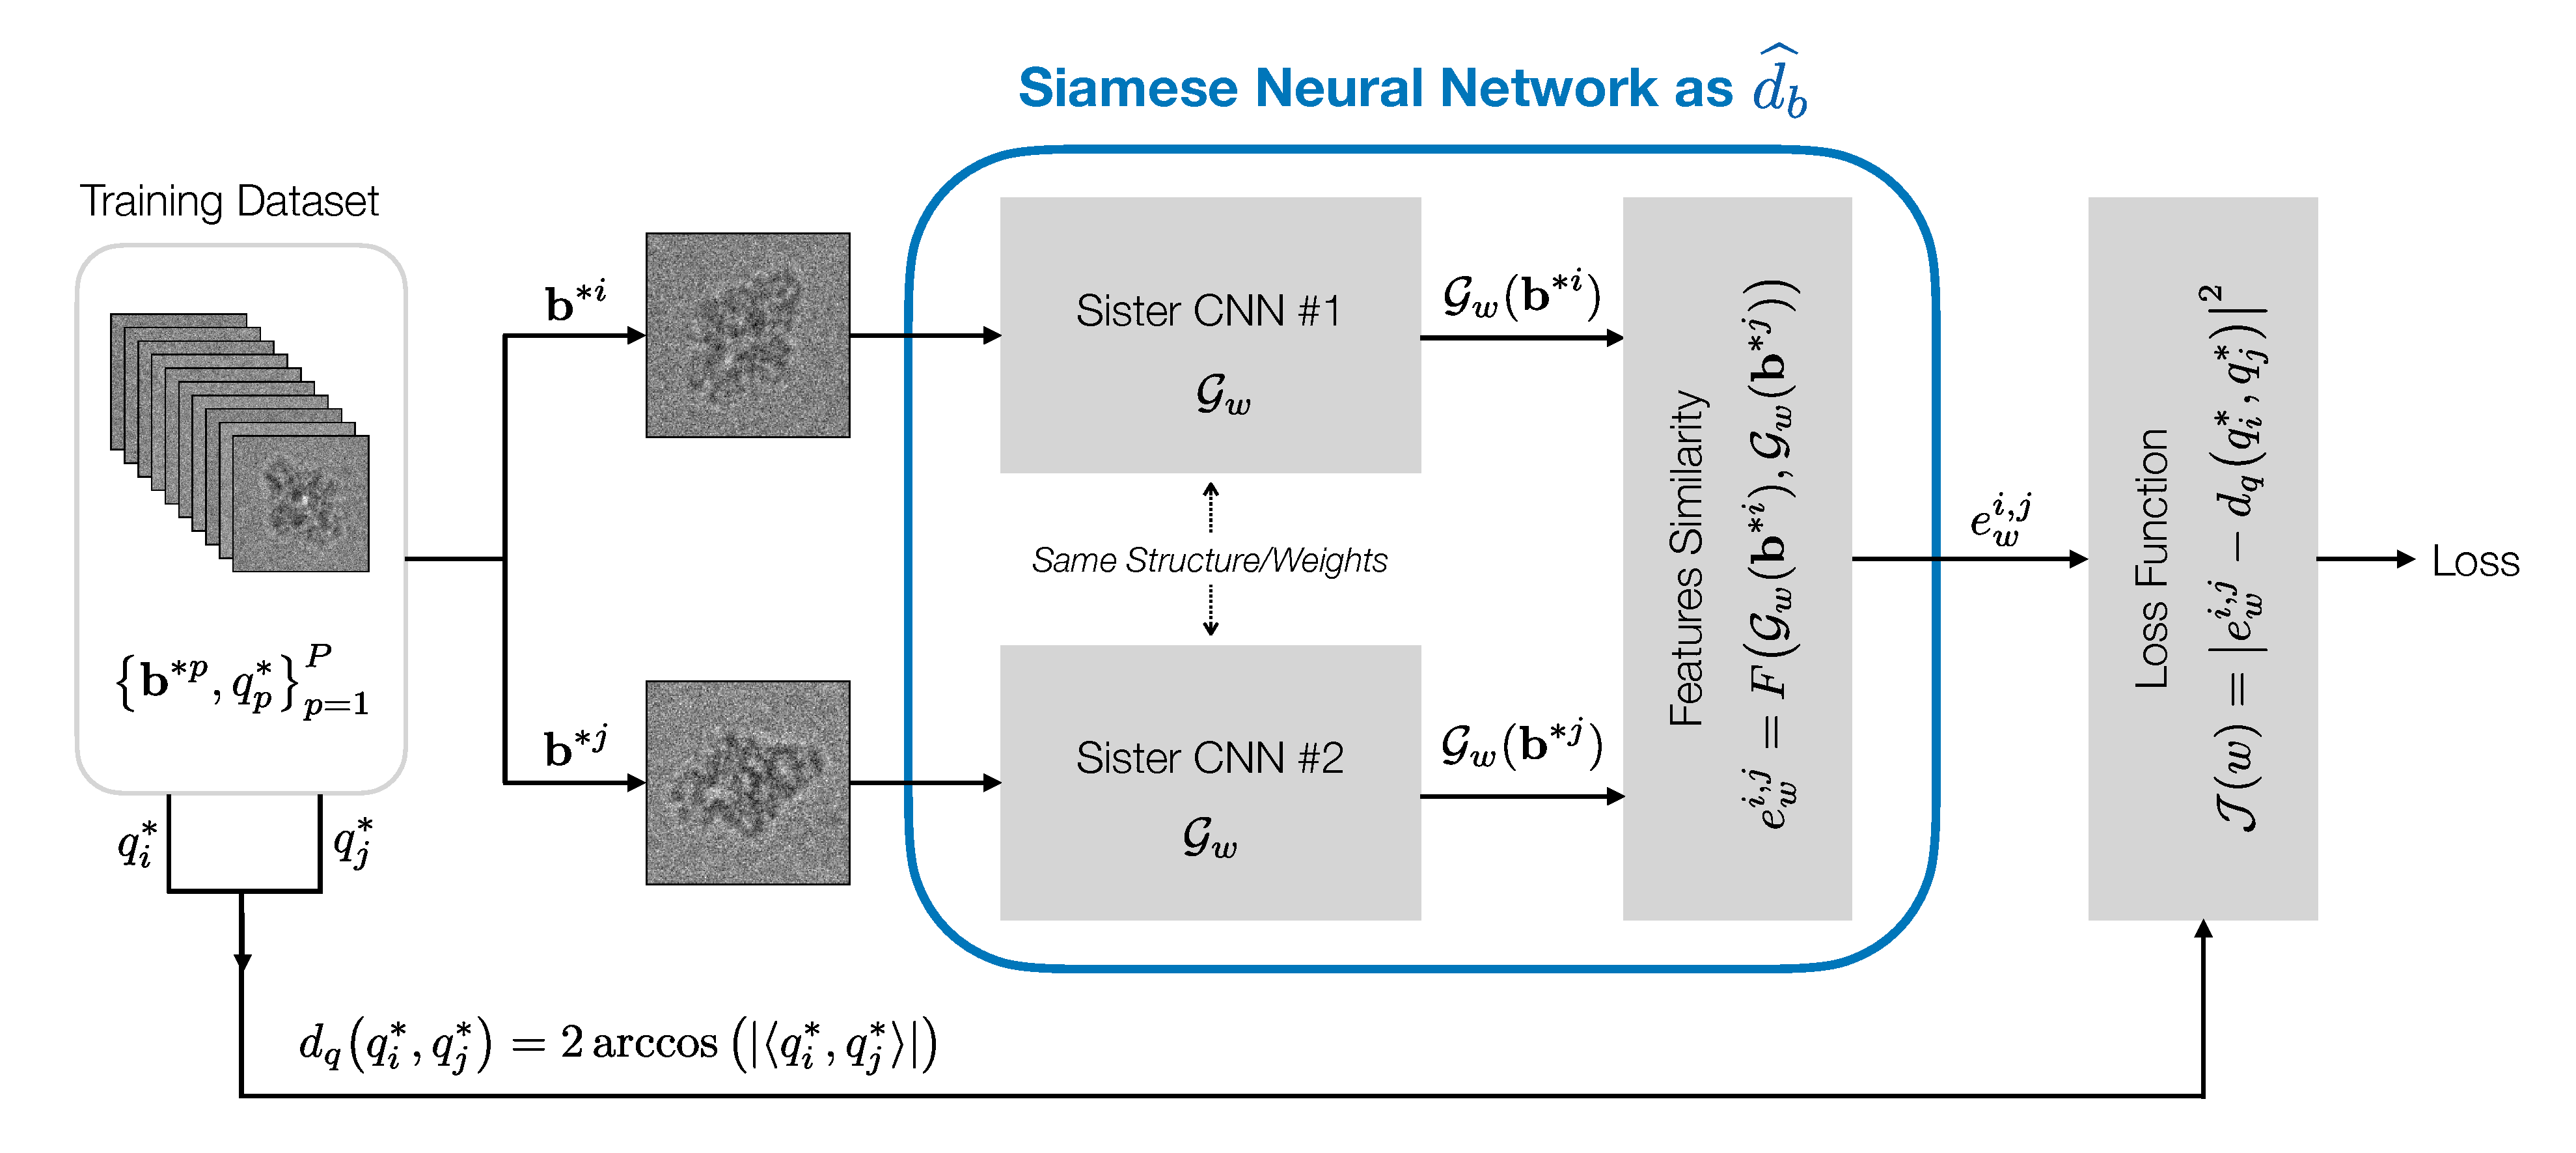
\includegraphics[width=\textwidth]{schematic_siamese}
    \caption{
        We are looking for a distance $d_p$ between projections that is an accurate estimator of the distance $d_q$ between their orientations.
        We propose to parameterize $d_p$ as a Siamese neural network (SiameseNN), trained on a synthetic dataset of $P \approx 10^3$ projections with associated orientation.
        \todo{Figure: feature distance (not similarity) $d_f$ is \eqnref{distance:projections}. Loss function is \eqnref{distance-learning}. "Same Structure/Weights" $\rightarrow$ "Same NN $\G$ and shared weights $w$".}
}
    \label{fig:schematic:distance-learning}
\end{figure}

\figref{schematic:distance-learning} illustrates the proposed learning paradigm.
\mdeff{Not a fan of this $*$ notation for the training data. I would just remove the $*$. Any problem with that? Other ideas?}
From a training dataset $\big\{ \mathbf{b}^{*p}, q^*_p \big\}_{p=1}^{P}$ made of $P$ projections $\p_i \in \R^{n_p}$ with associated orientation $q_i \in \U$, we learn the \textit{projection distance}
\begin{equation}
    \widehat{d}_b = \argmin_{d_b} \sum_{i,j} \left| d_b\big(\mathbf{b}^{*i},\mathbf{b}^{*j}\big) - d_q\big(q^*_i,q^*_j\big) \right|^2,
    \label{eqn:distance-learning}
\end{equation}
with $d_q$ defined in~\eqnref{distance:orientations}.
$d_b$ is parameterized as the Siamese neural network (SiameseNN)~\cite{chopra2005learning} 
\begin{equation}
    d_p(\p^i, \p^j) = d_f(\G_w(\p^i), \G_w(\p^j)),
    \label{eqn:distance:projections}
\end{equation}
where $\G_w$ is a convolutional neural network with weights $w$ that is trained to extract the most relevant features $\f_i \in \R^{n_f}$ from a projection $\p_i$.
$d_f$ is a distance in the feature space, which is often taken to be the Euclidean distance $d_f(\f_i, \f_j) = \Vert \f_i - \f_j \Vert_2$.
To facilitate the learning of a distance that respects the elliptic geometry of $\U$, we prefer $d_f = d_q$.

Evaluating the sum in \eqnref{distance-learning} requires $P^2$ distance evaluations.
As this is computationally infeasible for typical SPA datasets with $P \approx 10^4$ projections, we sample a subset of pairs.
In practice, \eqnref{distance-learning} is minimized by stochastic gradient descent (SGD) over small batches of pairs, with weight updates computed by back-propagation of the error.
% error / objective value

\subsection{Orientation recovery}\label{sec:method:orientation-recovery}
%\subsection{Orientation recovery from relative orientations}

With a trained estimator $\widehat{d}_b$, orientations are recovered from a set of projections $\big\{ \mathbf{p}_k \big\}_{k=1}^P$ as
\begin{equation}
    \big\{ \widehat{q}_k \big\}_{k=1}^P = \argmin_{q_i, q_j \in \U} \sum_{i,j} \left| \widehat{d}_b \left( \p_i, \p_j \right) - d_q\left(q_i,q_j\right) \right|^2.
    \label{eqn:orientation-recovery}
\end{equation}
Remark that the sole difference with~\eqnref{distance-learning} is that the minimization is over the projections $q_i$ rather than the distance $d_b$.

The sum in \eqnref{orientation-recovery} is again sampled for computational reasons.
A strategy, commonly employed by \todo{those classic algos}, that amounts to build and embed a sparse distance graph.
In practice, \eqnref{orientation-recovery} is again minimized by mini-batch SGD.
%We experimentally demonstrate in \secref{results:orientation-recovery:exact} that both approximations don't affect recovery performance.
